One of the major focuses of this work has been a completely new implementation of a program to generate and analyse $\mathrm{SU}(3)$ lattice gauge field configurations. As it is common practice in Lattice QCD numerical implementations, the program is split in three parts:
\begin{enumerate}
    \item \textit{Generation of Gauge Fields}: in this case it is done using an implementation of the Metropolis-Hastings algorithm using the Wilson gauge action;
    \item \textit{Computation of Lattice Observables}: this includes applying the gradient flow method, presented in \cref{sec:grad_flow}, to the gauge fields, as well as computing the energy density and the topological charge at every flow time; in other applications the computation of quark propagators and two- or three-point correlators are performed; 
    \item \textit{Computation of Derived Quantities}: mainly post analysis, computation of secondary observables and uncertainties. Resampling and autocorrelation analysis are crucial to Lattice QCD given the typically small size of the ensembles. 
\end{enumerate}
In this chapter we present the main features of the program that was developed to deal with the first two steps, which are the most interesting. The third step, the post analysis, which is a simpler calculation, did not require a very sophisticated implementation. \\
The problems are numerically very challenging and the calculations had to be performed on computing clusters. The programming language of choice was \cpp because of its high efficiency, high abstraction capabilities and for the easiness of the \mpi integration (a standard High Performance Computing (HPC) parallelization library). The analysis of data has been performed using \texttt{Python} and in particular relying heavily on its standard data science packages such as \texttt{numpy} and \texttt{pandas}.
  
\section{Generating Pure Gauge Fields} 
The task of generating lattice field configurations is extremely intense in terms of computational requirements. The case of full QCD with dynamical fermions is much more demanding than that of a Pure Gauge theory (no fermion determinants need to be computed, see \cref{sec:pathintegral}), but overall the latter calculation is still challenging. The main, and perhaps overwhelmingly simple, reason for this problem is the dimensionality. Dealing with a discretized space-time lattice, things tend to scale with powers of $2^4$, a trivial example is cutting in half the lattice spacing keeping a fixed total volume: this requires $16$ more points in the global lattice. \\
To get a better feeling of the algorithm we first have to look at what the basic object of the program is: the lattice. On a computer the number of double precision floating point numbers to be stored for a field configuration is given by
\begin{equation}
    \underbrace{N^3}_\text{spatial dimension} \times
    \underbrace{N_t}_\text{time dimension} \times
    \underbrace{4}_\text{links per site} \times 
    \underbrace{9}_\text{SU(3) matrix size} \times
    \underbrace{2}_\text{real and imaginary part}
\end{equation}
For example, if we choose $N=48,~N_t=96$ (which is the largest system considered in this work) the resulting configuration is $6115295232$ bytes large, that is $5.7$ GBytes.  The incredibly large size of the data to be handled limits greatly the possibility of simulating larger systems. \\
The basic element at each lattice site is a set of $4$ different $\mathrm{SU}(3)$ matrices, one for each dimension, these are the links variables described in \cref{sec:lattice_discretize}. Since the links with negative orientation are related to the ones with positive orientation by the adjoint operation, only the positively oriented ones are stored in memory.  

\subsection{The Metropolis-Hastings Algorithm}
The main algorithm that has been used to generate statistical ensembles of gauge field configurations is the Metropolis-Hastings algorithm. It is a widely popular Markov Chain Monte Carlo method to generate a sequence of random samples with a given probability distribution function \cite{metropolis_equation_1953}\cite{mhj}. \\
In general, a Markov Chain is a sequence of randomly chosen variables $X_1, X_2, \dots, X_t$, in our case a lattice field configuration, with the Markov property, that is: the probability of the step $t+1$ depends only on the variable $X_t$:
\beq
    P(X_{t+1} = x| X_1 = x_1, X_1 = x_2, \dots, X_t = x_t) = P(X_{t+1} = x|  X_t = x_t) .
\eeq 
In the case where the probabilities of moving from a state $X_i = i$ to a state $X_j = j$ is not known, the transition probability from the two states, $W(i\rightarrow j)$ can be split into two contributions: the probability $T(i \rightarrow j)$ for making the transition to state $j$ being in state $i$ and the  probability of accepting this transition $A(i \rightarrow j)$,
\beq
    W(i \rightarrow j) = A(i \rightarrow j)T(i \rightarrow j).
\eeq  
If a Probability Distribution Function (PDF) is known for the process, we can label the probability of a given state at a fixed time $w_i(t)$. The transition probability to a state $j$ at time $t+1$ is the sum of the transition probabilities of moving to state $j$ from state $i$ plus the probability of already being in state $j$ at time $t$ and rejecting to move to any other state:
\begin{align}
    w_{j} (t+1) &= \sum_i \left[ w_i(t)T(i\rightarrow j)A(i\rightarrow j) + w_j(t)T(j\rightarrow i)\left(1-A(j\rightarrow i)\right)  \right]\\\nonumber
    &=  w_j(t) + \sum_i \left[ w_i(t)T(i\rightarrow j)A(i\rightarrow j) -  w_j(t)T(j\rightarrow i)A(j\rightarrow i)  \right].
\end{align}
For large times $t$, when  equilibrium is reached, we require that $w_{j} (t+1) = w_{j} (t) = w_j$, and thus have:
\beq
    \sum_i w_iT(i\rightarrow j)A(i\rightarrow j) =  \sum_i w_jT(j\rightarrow i)A(j\rightarrow i).
\eeq 
Now, considering that the transition probability from a state $j$ to all other states must be normalized $\sum_i W(j\rightarrow i)  = \sum_i T(j\rightarrow i)A(j\rightarrow i) = 1$ we get:
\beq
    \sum_i w_iT(i\rightarrow j)A(i\rightarrow j) =  w_j.
\eeq 
At this point, the further constrain of ``detailed balance'' \cite{robert_monte_2004} is introduced, that is:
\beq
    w_iW(i\rightarrow j) =  w_j W(j\rightarrow i).
\eeq 
This condition means that at equilibrium every process is equilibrated by its reverse. We then have:
\beq
    \frac{w_i}{w_j} = \frac{W(i\rightarrow j)}{W(j\rightarrow i)} = \frac{T(i\rightarrow j)A(i\rightarrow j)}{T(j\rightarrow i)A(j\rightarrow i)}.
\eeq
Making the approximation that the transition probability between two states is the same independently of the direction of the transition: $T(i\rightarrow j) = T(j\rightarrow i)$. This is the so called brute-force approach. What we are left with is that the acceptance ratio of a move to a new state to be the ratio of the PDFs.  

The Metropolis-Hastings algorithm is used in such conditions. To sample the space of gauge configurations one performs the following procedure:
\begin{enumerate}
    \item Generate a candidate lattice gauge field configuration $\Lambda'$ at random starting from an initial one $\Lambda$. In practice this means to apply a random transformation to one of the link variables of $\Lambda$.
    \item Calculate the acceptance ratio. This is defined as the ratio $R$ of the PDFs of the candidate gauge field configuration and the initial one.
    \item Accept or Reject. Generate a uniform random number $u$ between $[0,1]$. 
    \begin{itemize}
        \item If $u \leq R$ accept the candidate configuration and set $\Lambda_{t+1} = \Lambda'$
        \item If $u > R$ reject the move and set $\Lambda_{t+1} = \Lambda$
    \end{itemize}
    \item Repeat steps $1$ to $3$.
\end{enumerate}

In the case of pure gauge fields, the probability distribution is:
\beq
\label{eq:PDF}
    P(U) = \frac{e^{S_G[U]}}{Z} = \frac{e^{S_G[U]}}{\int \D ~U e^{S_G[U]} },
\eeq
which is the exponential of the gluon Wilson Action over the path integral of the same quantity over all space (the partition function). Luckily, we only need ratios of PDFs so the partition function is never to be computed numerically. We can rewrite any expectation value of an operator on the lattice as:
\beq
    \langle O \rangle = \frac{\int \D U ~O[U] e^{S_G[U]}}{\int \D ~U e^{S_G[U]} } = \int  \D U ~ P(U) O[U],
\eeq 
which numerically becomes:
\beq
\langle O \rangle \approx \frac{1}{N} \sum_{i=1}^N O(U_i),
\eeq
where, as described in section \cref{sec:pathintegral}, $U_i$ are random configurations of a set chosen with the PDF of \cref{eq:PDF}. \\
Noting that, since we only care about ratios in the PDF, which turn out to be exponentials of the action difference between to configurations, an implementation of the Metropolis-Hastings algorithm to generate gauge field configurations can be written as: 
\begin{algorithm} [hbt!]
    \caption{Metropolis-Hastings Algorithm}\label{metropolis:algo}
    \begin{algorithmic}
    \State $\textit{configuration} \gets \text{initial configuration}$
    \For {$i < \textit{MonteCarloCycles}$}
        \For {$j < N_{corr}$}
            \For {$U$ in \textit{Lattice}}
                \State $\textit{newConfiguration}  \gets \text{randomMove}(U) + \textit{configuration}$  
                \State $\Delta S \gets \text{action} (\textit{newConfiguration}) - \text{action} (\textit{configuration})$
                \If {$\exp(-\Delta S) > random(0,1)$} 
                    \State $\textit{configuration} \gets \textit{newConfiguration}$
                \EndIf
            \EndFor 
        \EndFor 
        \State saveConfiguration$(configuration)$
    \EndFor
    \end{algorithmic}  
\end{algorithm} 

The actual implementation of this algorithm on discretized space-time is however not as trivial as it seems. Firstly, a definition of what is a ``random move'' in configuration space is needed, secondly an efficient way of computing the action difference is to be found.

The ensemble, on which observables can be computed, is created by saving to disk, in the form of a simple binary file containing all the data,  one configuration every $N_{corr}$ Monte Carlo updates. We need this in order to apply the gradient flow afterwards to the configurations and compute the observables we want. The choice of $N_{corr}$ turned out to be crucial for the autocorrelation of some observables, in particular the topological charge, see \cref{sec:testautocorr}.

\subsection{Sampling the Configuration Space}
\label{sec:randommatrix}
To use the Metropolis-Hastings algorithm we need to define a random walk in the space of gauge field configurations. In particular, we will use the Wilson Action for a lattice $\Lambda$:
\beq
S_G[U] = \frac{\beta}{3}\sum_{n\in\Lambda}\sum_{\mu<\nu} \text{Re} \Tr (\mathds{1} - P_{\mu\nu}(n)),
\eeq
which is defined on plaquettes $P_{\mu\nu}(n)$ and contains the parameter $\beta=6/g_0^2$ usually referred to as the inverse coupling. A random move in the configuration space can be seen as a random change of a single link of the lattice $\Lambda$. This change must be a unitary transformation in the $\mathrm{SU}(3)$ group, but not a completely random one as it should have a strong real diagonal component, making it close to an identity matrix and thus producing only a ``small change" on the link. \\
In order to generate such a transformation we use three random $\mathrm{SU}(2)$ matrices that are as well ``close to unity''. A recipe for generating these matrices is found in \cite{gattringer_quantum_2010}. We consider three $2\times 2$ unitary matrices $R_2,S_2$ and $T_2$:
\beq
    R_2 = \begin{pmatrix}
        r_{11} & r_{12} \\ r_{21} & r_{22} 
    \end{pmatrix},
    ~~~~~~~
    S_2 = \begin{pmatrix}
        s_{11} & s_{12} \\ s_{21} & s_{22} 
    \end{pmatrix},
    ~~~~~~~
    T_2 = \begin{pmatrix}
        t_{11} & t_{12} \\ t_{21} & t_{22} 
    \end{pmatrix},
\eeq
The elements of the matrix are to be random, but with a controlled spread around the identity matrix. One starts by selecting four random numbers $r_0$, $\vec{r}$ (the latter is a three component vector) between $(-\frac{1}{2},\frac{1}{2})$. 
Then a ``spread parameter'' $\epsilon$ is introduced, which controls how much to weight the off-diagonal terms. The random variables are scaled according to:
\beq
    x_0 = sign(r_0)\sqrt{1-\epsilon^2}~~~~~~\vec{x}, = \epsilon \frac{\vec{r}}{|\vec{r}|},
\eeq
and these four coefficients, together with the generators of the $\mathrm{SU}(2)$ group (the Pauli matrices)  are used to build the element of the group:
\beq
U = x_0\mathds{1} + i\vec{x}\cdot\vec{\sigma} = \begin{pmatrix}
    u_{11} & u_{12} \\ u_{21} & u_{22} 
\end{pmatrix},
\eeq
One then embeds these $\mathrm{SU}(2)$ matrices in three $\mathrm{SU}(3)$ matrices by mapping them as:
\beq
    R = \begin{pmatrix}
        r_{11} & r_{12} & 0\\ r_{21} & r_{22} & 0 \\ 0 & 0 & 1 
    \end{pmatrix},
    ~~~~~~~
    S = \begin{pmatrix}
        s_{11} & 0 & s_{12} \\ 0 & 1 & 0 \\ s_{21} & 0 & s_{22} 
    \end{pmatrix},
    ~~~~~~~
    T = \begin{pmatrix}
        1 & 0 & 0 \\ 0 & t_{11} & t_{12} \\ 0 & t_{21} & t_{22} 
    \end{pmatrix}.
\eeq
These three matrices are clearly members of the $\mathrm{SU}(3)$ group and so is their product $X = RST$, which is used as the ``random move'' in the Metropolis-Hastings algorithm. We thus have defined a recipe for numerically generating random transformations, the key element for our algorithm.

\subsection{Efficient Action Difference Calculation}
An additional element that is needed in the Metropolis-Hastings algorithm is the action difference $\Delta S$, used in evaluating the ratio of the PDFs between configurations. When a random transformation $U_\mu(n) \rightarrow U'_\mu(n) = XU_\mu(n)$ is applied on a single link of the lattice, the total change in the action only depends on the plaquettes that contain the considered link variable. In four dimensions there are 12 such elements. The action difference for a single gauge link is then:
\beq
    \Delta S(n) = S[U'_\mu(n)] - S[U_\mu(n)]  = -\frac{\beta}{N} \text{Re}~ Tr \left( [U'_\mu(n) - U_\mu(n)] A[U_\mu(n)]\right),
\eeq
where $A[U_\mu(n)]$ is the sum of the ``staples" of the link $U_\mu(n)$. They are the constant three sides of the plaquettes that contain $U_\mu(n)$:
\begin{align}
    \label{eq:staples}
    A[U_\mu(n)] = \sum_{\nu\neq\mu} &\bigg[ U_{\nu}(n+\mu)U_{-\mu}(n+\mu+\nu)U_{-\nu}(n+\nu) \\\nonumber
    +  &U_{-\nu}(n+\mu)U_{-\mu}(n+\mu-\nu)U_{\nu}(n-\nu)  \bigg]
\end{align}
An intuitive pictorial representation is given in \cref{fig:staples}.

\begin{figure}[!htb]
    \centering

    \begin{tikzpicture}[scale=0.7]

        \pgfmathsetmacro\len{1.2};
        \pgfmathsetmacro\startx {-6};
        \pgfmathsetmacro\startxx {-5};
        \pgfmathsetmacro\startxxx {-3};
        \pgfmathsetmacro\startxxxx {0};

        \pgfmathsetmacro\starttxxxx {4.5};
        \pgfmathsetmacro\starttx {4};
        \pgfmathsetmacro\starttxx {4.8};
        \pgfmathsetmacro\starttxxx {6.8};
        \pgfmathsetmacro\starty {0};
        \pgfmathsetmacro\startty {0};

        \node [left] (a) at  (\startx, \starty) {$S[U_\mu](n) = \sum_{\nu\neq\mu}$}; 
         
        \draw (-5,-2) to [round left paren ] (-5,2);

        % ++
        \draw[->-=.7, >=latex,red] (\startxx,\starty) to (\startxx+\len,\starty);
        \draw[->-=.7, >=latex] (\startxx+\len,\starty) to  (\startxx+\len,\starty+\len);
        \draw[->-=.7, >=latex] (\startxx+\len,\starty+\len) to (\startxx,\starty+\len);
        \draw[->-=.7, >=latex] (\startxx,\starty+\len) to (\startxx, \starty);
 
        \node (b) at (-3.4, \starty) {$+$}; 
        %+-
        \draw[->-=.7, >=latex,red] (\startxxx,-\starty) to (\startxxx+\len,-\starty);
        \draw[->-=.7, >=latex] (\startxxx+\len,-\starty) to  (\startxxx+\len,-\starty-\len);
        \draw[->-=.7, >=latex] (\startxxx+\len,-\starty-\len) to (\startxxx,-\starty-\len);
        \draw[->-=.7, >=latex] (\startxxx,-\starty-\len) to (\startxxx, -\starty);
        \draw (-1.7,-2) to [round right paren ] (-1.7,2); 

       \node (c) at  (-0.7, \starty) {$=$}; 

        \draw[->-=.7, >=latex, red] (\startxxxx,\starty) to (\startxxxx+\len,\starty); 

       \node [right](f) at  (1.4, \starty) {$\times \sum_{\nu\neq\mu} $}; 
         
        \draw (\starttxxxx,-2) to [round left paren ] (\starttxxxx,2);

        % ++
        \draw[->-=.7, >=latex] (\starttxx+\len,\startty) to  (\starttxx+\len,\startty+\len);
        \draw[->-=.7, >=latex] (\starttxx+\len,\startty+\len) to (\starttxx,\startty+\len);
        \draw[->-=.7, >=latex] (\starttxx,\startty+\len) to (\starttxx, \startty);
 
        \node (d) at  (6.4, \startty) {$+$}; 
        %+-
        \draw[->-=.7, >=latex] (\starttxxx,-\startty-\len) to (\starttxxx,-\startty);
        \draw[->-=.7, >=latex] (\starttxxx+\len,-\startty) to  (\starttxxx+\len,-\startty-\len);
        \draw[->-=.7, >=latex] (\starttxxx+\len,-\startty-\len) to (\starttxxx,-\startty-\len);
        \draw (8.2,-2) to [round right paren ] (8.2,2); 

    \end{tikzpicture}

    \capt{Schematic representation of the symmetric definition of action around a single link $S[U_\mu](n)$ expressed as a function of the staples. The link in red is the one that is being considered for the action, $U_\mu(n)$. On the left side there is the action defined as the sum of all the plaquettes containing $U_\mu(n)$. On the right side the link $U_\mu(n)$ is factored out to show the meaning of the staples $A[U_\mu(n)]$. The sum on the right-hand side is $A[U_\mu(n)]$ as defined in \cref{eq:staples}.}
    \label{fig:staples}
\end{figure}


\subsection{Updates Strategies}
\label{sec:update}
There is now some arbitrariness in what is defined as a Monte Carlo update, or cycle. In this work we call an update the procedure outlined in \cref{metropolis:update}. 

\begin{algorithm}[bht!]
    \caption{Metropolis-Hastings Update}\label{metropolis:update}
    \begin{algorithmic}[1]
    \For {$x,\mu$}
        \State $A \gets computeStaples(n,\mu)$     
        \For {$i < N_{hits}$}
            \State $U_{new}(n,\mu)  \gets X\cdot U(n,\mu)$  
            \State $\Delta S \gets (U_{new}(n,\mu)  - U(n,\mu) )\cdot A$
            \If {$\exp(-realTrace(\Delta S)) > random(0,1)$} 
                \State $U(n,\mu)  \gets U_{new}(n,\mu)$
            \EndIf
        \EndFor
    \EndFor
\end{algorithmic}
\end{algorithm}

These updates are the ones we consider when we refer to Monte Carlo cycles (MC cycles) in the context of thermalization and autocorrelation time, for example. Note that each update includes a loop over all links on the lattice and that every link is ``hit" (tentatively updated) $N_{hits}$ times before moving to the next one. This is done for computational efficiency, because evaluating the staples is the most expensive part of the algorithm. Once $A[U_\mu(n)]$ is calculated for a link, the result is used to attempt multiple updates on the same link variable. It can also be shown that if $N_{hits}$ is sufficiently large the algorithm becomes equivalent to the heatbath algorithm \cite{gattringer_quantum_2010}. 

The order in which the links in the lattice are visited is also arbitrary. The simplest way, that is iterating on the links as they are stored in memory, has been adopted. This however might have impacted the autocorrelation of the system, not allowing significant modification to the system as an update depends on the neighbors. An alternative choice is a checkerboard pattern, which has potential benefits to the autocorrelation time of the observables as well as on the performance, as it allows for better communication patterns in the case of a parallelized code. 

\subsection{Parallelization Scheme}
\label{sec:para_gen}
Given the size of the lattice (the total number of sites in this work is from $|\Lambda| \approx 10^5$ to $|\Lambda|\approx 10^7$), it is almost necessary to split the computation of the updates on more than one processors. The most direct way is to divide the lattice into sub-blocks, or sub-lattices, and have each process handle its portion of the field alone. \\
In an operative way, given a lattice of size $(N_x, N_y, N_z, N_t)$ each space-time dimension is split into even portions, of size $(S_x, S_y, S_z, S_t)$ and mapped on $N_{procs}$ processors, having that:
\beq
N_{procs} = \frac{S_x}{N_x} \times \frac{S_y}{N_y} \times \frac{S_z}{N_z}  \times \frac{S_t}{N_t}.
\eeq 
A unique mapping can be performed from the ``local'' coordinates of a lattice site in one of the sub-blocks to the ``global" coordinates once the position of the sub-lattice is known. In practice this can be done through the aid of the unique identifier of the processor that is given by the parallelization library. In particular, the Message Passing Interface (\texttt{MPI}) has a built-in function to map processors into a grid of arbitrary dimensions and size, called \texttt{MPI\_CartCoord\_Create}. The utility also allows for the easy identification of the rank (the jargon term for the unique identifier of a processor) of the nearest neighbors. Using this tools one can manage the distribution of the total lattice into $N_{procs}$ sub-lattices. \\
However, the plaquette $P_{\mu\nu}(n)$ of a lattice site $n$, that enters the action difference definition, depends on link variables located at neighboring sites, this is clear by looking at the definition found in \cref{plaquette}. This implies that when updating a link on the edge of a sub-lattice, information about another block is needed. Here is where \texttt{MPI} comes in use, substituting the usual periodic boundary conditions that are used in the calculations with periodic communication patterns between the processors. For this particular problem we decided to use a point to point communication scheme, the use of periodic boundary conditions allowed also for non-blocking communications, in particular the collective geometry based scheme shown in \cref{fig:subblocks} has been implemented. 

\newif\ifcuboidshade
\newif\ifcuboidemphedge

\tikzset{
  cuboid/.is family,
  cuboid,
  shiftx/.initial=0,
  shifty/.initial=0,
  dimx/.initial=3,
  dimy/.initial=3,
  dimz/.initial=3,
  scale/.initial=1,
  densityx/.initial=1,
  densityy/.initial=1,
  densityz/.initial=1,
  rotation/.initial=0,
  anglex/.initial=0,
  angley/.initial=90,
  anglez/.initial=225,
  scalex/.initial=1,
  scaley/.initial=1,
  scalez/.initial=0.5,
  front/.style={draw=black,fill=white},
  top/.style={draw=black,fill=white},
  right/.style={draw=black,fill=white},
  shade/.is if=cuboidshade,
  shadecolordark/.initial=black,
  shadecolorlight/.initial=white,
  shadeopacity/.initial=0.15,
  shadesamples/.initial=16,
  emphedge/.is if=cuboidemphedge,
  emphstyle/.style={thick},
}

\newcommand{\tikzcuboidkey}[1]{\pgfkeysvalueof{/tikz/cuboid/#1}}

% Commands
\newcommand{\tikzcuboid}[1]{
    \tikzset{cuboid,#1} % Process Keys passed to command
  \pgfmathsetlengthmacro{\vectorxx}{\tikzcuboidkey{scalex}*cos(\tikzcuboidkey{anglex})*28.452756}
  \pgfmathsetlengthmacro{\vectorxy}{\tikzcuboidkey{scalex}*sin(\tikzcuboidkey{anglex})*28.452756}
  \pgfmathsetlengthmacro{\vectoryx}{\tikzcuboidkey{scaley}*cos(\tikzcuboidkey{angley})*28.452756}
  \pgfmathsetlengthmacro{\vectoryy}{\tikzcuboidkey{scaley}*sin(\tikzcuboidkey{angley})*28.452756}
  \pgfmathsetlengthmacro{\vectorzx}{\tikzcuboidkey{scalez}*cos(\tikzcuboidkey{anglez})*28.452756}
  \pgfmathsetlengthmacro{\vectorzy}{\tikzcuboidkey{scalez}*sin(\tikzcuboidkey{anglez})*28.452756}
  \begin{scope}[xshift=\tikzcuboidkey{shiftx}, yshift=\tikzcuboidkey{shifty}, scale=\tikzcuboidkey{scale}, rotate=\tikzcuboidkey{rotation}, x={(\vectorxx,\vectorxy)}, y={(\vectoryx,\vectoryy)}, z={(\vectorzx,\vectorzy)}]
    \pgfmathsetmacro{\steppingx}{1/\tikzcuboidkey{densityx}}
  \pgfmathsetmacro{\steppingy}{1/\tikzcuboidkey{densityy}}
  \pgfmathsetmacro{\steppingz}{1/\tikzcuboidkey{densityz}}
  \newcommand{\dimx}{\tikzcuboidkey{dimx}}
  \newcommand{\dimy}{\tikzcuboidkey{dimy}}
  \newcommand{\dimz}{\tikzcuboidkey{dimz}}
  \pgfmathsetmacro{\secondx}{2*\steppingx}
  \pgfmathsetmacro{\secondy}{2*\steppingy}
  \pgfmathsetmacro{\secondz}{2*\steppingz}
  \ifthenelse{\equal{\dimx}{1}}
    {\foreach \x in {\steppingx,...,\dimx}}
    {\foreach \x in {\steppingx,\secondx,...,\dimx}}
  {     \ifthenelse{\equal{\dimy}{1}}
    {\foreach \y in {\steppingy,...,\dimy}}
    {\foreach \y in {\steppingy,\secondy,...,\dimy}}
    {   \pgfmathsetmacro{\lowx}{(\x-\steppingx)}
      \pgfmathsetmacro{\lowy}{(\y-\steppingy)}
      \filldraw[cuboid/front] (\lowx,\lowy,\dimz) -- (\lowx,\y,\dimz) -- (\x,\y,\dimz) -- (\x,\lowy,\dimz) -- cycle;
    }
    }
    \ifthenelse{\equal{\dimx}{1}}
    {\foreach \x in {\steppingx,...,\dimx}}
    {\foreach \x in {\steppingx,\secondx,...,\dimx}}
  { \ifthenelse{\equal{\dimz}{1}}
    {\foreach \z in {\steppingz,...,\dimz}}
    {\foreach \z in {\steppingz,\secondz,...,\dimz}}
    {   \pgfmathsetmacro{\lowx}{(\x-\steppingx)}
      \pgfmathsetmacro{\lowz}{(\z-\steppingz)}
      \filldraw[cuboid/top] (\lowx,\dimy,\lowz) -- (\lowx,\dimy,\z) -- (\x,\dimy,\z) -- (\x,\dimy,\lowz) -- cycle;
        }
    }
    \ifthenelse{\equal{\dimy}{1}}
    {\foreach \y in {\steppingy,...,\dimy}}
    {\foreach \y in {\steppingy,\secondy,...,\dimy}}
  { \ifthenelse{\equal{\dimz}{1}}
    {\foreach \z in {\steppingz,...,\dimz}}
    {\foreach \z in {\steppingz,\secondz,...,\dimz}}
    {   \pgfmathsetmacro{\lowy}{(\y-\steppingy)}
      \pgfmathsetmacro{\lowz}{(\z-\steppingz)}
      \filldraw[cuboid/right] (\dimx,\lowy,\lowz) -- (\dimx,\lowy,\z) -- (\dimx,\y,\z) -- (\dimx,\y,\lowz) -- cycle;
    }
  }
  \ifcuboidemphedge
    \draw[cuboid/emphstyle] (0,\dimy,0) -- (\dimx,\dimy,0) -- (\dimx,\dimy,\dimz) -- (0,\dimy,\dimz) -- cycle;%
    \draw[cuboid/emphstyle] (0,\dimy,\dimz) -- (0,0,\dimz) -- (\dimx,0,\dimz) -- (\dimx,\dimy,\dimz);%
    \draw[cuboid/emphstyle] (\dimx,\dimy,0) -- (\dimx,0,0) -- (\dimx,0,\dimz);%
    \fi

    \ifcuboidshade
    \pgfmathsetmacro{\cstepx}{\dimx/\tikzcuboidkey{shadesamples}}
    \pgfmathsetmacro{\cstepy}{\dimy/\tikzcuboidkey{shadesamples}}
    \pgfmathsetmacro{\cstepz}{\dimz/\tikzcuboidkey{shadesamples}}
    \foreach \s in {1,...,\tikzcuboidkey{shadesamples}}
    {   \pgfmathsetmacro{\lows}{\s-1}
        \pgfmathsetmacro{\cpercent}{(\lows)/(\tikzcuboidkey{shadesamples}-1)*100}
        \fill[opacity=\tikzcuboidkey{shadeopacity},color=\tikzcuboidkey{shadecolorlight}!\cpercent!\tikzcuboidkey{shadecolordark}] (0,\s*\cstepy,\dimz) -- (\s*\cstepx,\s*\cstepy,\dimz) -- (\s*\cstepx,0,\dimz) -- (\lows*\cstepx,0,\dimz) -- (\lows*\cstepx,\lows*\cstepy,\dimz) -- (0,\lows*\cstepy,\dimz) -- cycle;
        \fill[opacity=\tikzcuboidkey{shadeopacity},color=\tikzcuboidkey{shadecolorlight}!\cpercent!\tikzcuboidkey{shadecolordark}] (0,\dimy,\s*\cstepz) -- (\s*\cstepx,\dimy,\s*\cstepz) -- (\s*\cstepx,\dimy,0) -- (\lows*\cstepx,\dimy,0) -- (\lows*\cstepx,\dimy,\lows*\cstepz) -- (0,\dimy,\lows*\cstepz) -- cycle;
        \fill[opacity=\tikzcuboidkey{shadeopacity},color=\tikzcuboidkey{shadecolorlight}!\cpercent!\tikzcuboidkey{shadecolordark}] (\dimx,0,\s*\cstepz) -- (\dimx,\s*\cstepy,\s*\cstepz) -- (\dimx,\s*\cstepy,0) -- (\dimx,\lows*\cstepy,0) -- (\dimx,\lows*\cstepy,\lows*\cstepz) -- (\dimx,0,\lows*\cstepz) -- cycle;
    }
    \fi 

  \end{scope}
}

\makeatother


\begin{figure}[!hbt]
\centering
\begin{tikzpicture}[scale=0.7]

\tikzcuboid{dimx=1,dimy=1,dimz=1,shiftx=-400, scale=4};
\tikzcuboid{dimx=4,dimy=4,dimz=4,shiftx=4,scale=1};
 
\node (A) at (-7, 1) {};
\node (B) at (-4, 1) {};
\draw[-latex,thick] (A) to (B); 
\draw [-latex] (-9.5,2.5) arc [start angle=-45, end angle=225, x radius=4.5cm, y radius=1.3cm];

\draw [-latex] (2.95, 2.1) arc [start angle=-45, end angle=225, x radius=3cm, y radius=1.3cm];


\node (C) at (-12.5, 5.5) {Periodic Boundary Conditions};
\node (D) at (1.6, 5.5) {Periodic Communication Pattern};

\draw [black,decorate,decoration={brace,amplitude=5pt,mirror}](-1.35,-1.55) -- (-0.15,-1.55) node[black,midway,yshift=-0.5cm] {\footnotesize $s_x$ Lattice Sites};

\draw [black,decorate,decoration={brace,amplitude=5pt,mirror}](-15.5,-1.55) -- (-11.5,-1.55) node[black,midway,yshift=-0.5cm] {\footnotesize $n_x$ Lattice Sites};

\draw[-latex] (-0.55, 2.1) to (0.05, 2.1);
\draw[-latex] (-0.55 + 1, 2.1) to (0.05 + 1., 2.1);
\draw[-latex] (-0.55 + 2, 2.1) to (0.05 + 2, 2.1);

\draw[-latex] (-0.55, 1.1) to (0.05, 1.1);
\draw[-latex] (-0.55 + 1, 1.1) to (0.05 + 1., 1.1);
\draw[-latex] (-0.55 + 2, 1.1) to (0.05 + 2, 1.1);

\draw[-latex] (-0.55, 0.1) to (0.05, 0.1);
\draw[-latex] (-0.55 + 1, 0.1) to (0.05 + 1., 0.1);
\draw[-latex] (-0.55 + 2, 0.1) to (0.05 + 2, 0.1);

\draw[-latex] (-0.55, -0.9) to (0.05, -0.9);
\draw[-latex] (-0.55 + 1, -0.9) to (0.05 + 1., -0.9);
\draw[-latex] (-0.55 + 2, -0.9) to (0.05 + 2, -0.9);

\end{tikzpicture}
\label{fig:subblocks}
\capt{Schematic representation, in just 3 dimesnions, of the splitting of the lattice into sub-lattices. The full system, which has periodic boundary conditions to emulate infinite volumes, is split into sub-blocks. These smaller regions of spacetime do not have periodic boundary conditions, but share faces with the neighboring blocks. To reproduce the periodicity, the communication pattern between the sub-lattices is made periodic, meaning that all sub-block that are aligned in one direction cyclically share faces with the neighbors.}
\end{figure}
 

When computing the staples, two links need to be fetched from the neighboring sites, since all processors are synchronized, when one processor is in need of these link variables one of its neighbors is requesting the corresponding links from it. The \texttt{SendRecv} function of \texttt{MPI} is exactly what is needed: it automatically handles, in the most efficient way, multiple data transfer between processors in situations when a single core needs to send and receive from different ranks. \\ 
Note that the communication is relevant only for the computation of the staples, this is another argument in favor of performing multiple hits on a link at every update. \\
It is clear to see that the algorithm can be affected by large communication overhead problems. If the sub-blocks are too small, then most of the time would be spent on sending and receiving links from the neighbors. This causes the execution time to depend not linearly on the number of processors, instead the relation flattens at some value given by the communication overhead.

\subsection{Summary of the Parameters for Generating Configurations}
In total the algorithm we presented for generating pure gauge field configurations (using only the Wilson gluonic action) has four parameters as inputs. Of these, only one defines the physics of the system, the others have to be set and optimized in order to improve the acceptance ratio of the metropolis algorithm and the autocorrelation time of the observables computed on the generated configurations. A summary is reported in \cref{MC:params}
 
\begin{table}[!htb]
    \capt{Parameters for the Monte Carlo generation of Yang-Mills gauge field \\configurations via the Metropolis-Hastings Algorithm}
    \begin{center}
\begin{tabular}{cl}
    Parameter & Description\\\hline
    $\beta$ & Coupling parameter of the Wilson Action\\
    $\epsilon$ & ``Spread'' of the random $\mathrm{SU}(3)$ elements for the updates\\
    $N_{corr}$ & Number of updates between every saved configuration (observable measurement)\\
    $N_{hits}$ & Number of of "hits" per link at every update, with constant staple 
\end{tabular}
\label{MC:params}
\end{center}
\end{table}
 
\section{Gradient Flow of Gauge Configurations}
To study the flow time dependence of the observables a numeric implementation of \cref{lattice:flow} is needed. The main challenge that this problem poses is how to numerically integrate the flow equation on the lattice while preserving the $\mathrm{SU}(3)$ Lie Group structure of the field through the numerical procedure. The problem is solved by using the so called Structure-Preserving Runge-Kutta Methods, in particular the Runge-Kutta Munthe-Kaas (RK-MK) method that is designed to integrate first order ODE on a manifold \cite{munthe-kaas_runge-kutta_1998,munthe-kaas_lie-butcher_1995,celledoni_introduction_2014}. \\
In \cref{algo:flow} the general scheme of the program to flow the gauge field configurations from time $t_f=0$ to $t_f^{MAX}$ in steps of size $\epsilon$ is outlined.
\begin{algorithm}[bht!]
    \caption{Gradient Flow}\label{algo:flow}
    \begin{algorithmic}[1]
    \For {\textit{conf} in $ensemble$}
        \State \textit{conf} \gets readInputFile()     
        \For {$t_f = 0,~ t_f < t_f^{MAX}$}
            \State \textit{conf} \gets flowStep(\textit{conf})
            \State computeObservables(\textit{conf}) 
            \State $t_f$ \gets $t_f + \epsilon$
        \EndFor
    \EndFor
\end{algorithmic}
\end{algorithm}

The main idea is to loop over all the configurations in an ensemble, provided as a set of input files, and for each of them numerically integrate the gradient flow equation \cref{eq:flow_cont} in steps of $\epsilon$ (a dimensionless small step parameter). By using an explicit RK method, only one lattice is stored in memory at a time, and is updated at every iteration. At each step, the expectation values of all the desired observables are computed and their value stored to file for further analysis.

\subsection{Numerical Integration of the Flow Equation}
The problem of the gradient flow can be defined in more general terms as:
\beq
    \dot{V}_t =  Z(V_t)V_t.
\eeq
here $V_t$ is an element of a Lie group $\mathcal{G}$ and $Z(V_t)$ is an algebra-valued function, in our case we have:
\beq 
Z(V_t) = -g_0^2\partial_\mu S_G[V_t].
\label{eq:flow_action}
\eeq
The general ansatz for the RK-MK method is to write the integration step, with $\epsilon$ being the integration step, as:
\beq
    V_{t+\epsilon} =  \exp[\epsilon\Omega(V_t)] V_t,
\eeq
where $\Omega(V_t)$ is a linear combination of $Z(V_t + \epsilon c_i)$, with $c_i$ the RK coefficients, and of their commutators. Following the suggestion of \cite{luscher_properties_2010} the third order integration scheme  has been used:
\begin{align}
    \label{eq:integrator}
    &W_0 = V_t\\\nonumber
    &W_1 = \exp\left[ \frac{1}{4}Z_0 \right] W_0 \\\nonumber
    &W_2 = \exp\left[ \frac{8}{9}Z_1 - \frac{17}{36}Z_0 \right] W_1\\\nonumber
    &V_{t+\epsilon} = \exp\left[ \frac{3}{4}Z_2 - \frac{8}{9}Z_1 + \frac{17}{36}Z_0\right] W_2,
\end{align}
where the shorthand notation $Z_i = i\epsilon Z(W_i)$ has been introduced. The choice of the coefficients for the Butcher's tableu \cite{_numerical_????} of the RK method is made in order to satisfy the requirements for a third order RK integrator and to cancel the commutator terms in $\Omega(V_t)$ when expanding it with the Baker-Campbell-Husdorff formula. \\
The choice of the integration step size $\epsilon$ as been motivated by the results found in \cite{ce_testing_2015}. The article suggests that for an integrator of third order the choice of $\epsilon=0.01-0.02$ is sufficient to keep the numerical error under control.\\
What is then left to define are the derivative of the action at a given lattice site and the numerical exponentiation of a member of the $\mathfrak{su}(3)$ algebra, which returns an $\mathrm{SU}(3)$ element.

\subsection{The Action Derivative}
The differential operator acting on an algebra-valued function $f(U)$ in a Lie group is defined, in terms of the generators $t^a$, as:
\beq
    \partial_{\mu,x}^a f(U) = \frac{d}{ds} f(e^{sX}U) \bigg\rvert_{s=0},~~~~~\text{with} ~~~X(\mu,x) = t^a \delta_{x,y}\delta_{\mu,\nu} .
\eeq
In practice this operator leaves unchanged all the links except the one that is being derivated. When considering the action in \cref{eq:flow_action} and recalling the definition of staples, \cref{eq:staples}, we have:
\beq
\partial_{\mu,x}^a S_G(U_\mu(x)) = -\frac{2}{g_0^2} \sum_{x \in \Lambda} \sum_{\mu \neq \nu} \text{Re}\Tr (1-P_{\mu\nu}) = -\frac{2}{g_0^2}  \text{Re}\Tr (t^a U_\mu(x) A[U_\mu(x)]).
\eeq
Defining $\Omega_\mu(x) = U_\mu(x) A[U_\mu(x)]$ and summing over all generators one has:
\beq
g_0^2\partial_{\mu,x} S_G(U_\mu(x)) = 2 t^a  \text{Re}\Tr (t^a \Omega_\mu(x)) = t^a \Tr (t^a (\Omega_\mu(x) - \Omega^\dagger_\mu (x)) .
\eeq
Invoking now the fact that any $3\times3$ matrix can be expanded as $M = \frac{1}{3} \Tr M - 2 t^a\Tr(t^aM)$, we can rewrite the equation as:
\beq
g_0^2\partial_{\mu,x} S_G(U_\mu(x)) = \frac{1}{2} \left(\Omega_\mu(x) - \Omega^\dagger_\mu (x) \right) -  \frac{1}{6} \Tr \left(\Omega_\mu(x) - \Omega^\dagger_\mu (x) \right).
\eeq
This is our final expression for the action derivative. It should be noticed that computing this term is not anymore complex than computing the action difference for the gauge field configuration generation case, as in both cases the most complicated object to calculate on the lattice is the sum of the staples $A[U_\mu(x)]$. We can notice as well that the derivative is always a traceless hermitean matrix, thus an element of $\mathfrak{su}(3)$ as expected.

\subsection{Exponential of an $\mathfrak{su}(3)$ Element}
\label{sec:exponential}
The last thing to define from \cref{eq:integrator} is how to exponentiate the action derivative, that apperas in the form $\exp[i\epsilon Z(W_i)]$. Following \cite{morningstar_analytic_2004} we provide a numerical recipe for taking the exponential function of a traceless hermitean $3\times3$ matrix. The key idea is to use the Cayley-Hamilton theorem, that states that every matrix is a zero of its characteristic polynomial:
\beq
    Q^3 - c_1 Q - c_0\mathds{1} = 0,~~~~~\text{with}~~c_0 = \det Q = \frac{1}{3}(Q^3),~~~c_1 =\frac{1}{2}(Q^2).
\eeq
The exponential of $iQ$ can then be written as:
\beq    
e^{iQ} = f_0\mathds{1} + f_1Q+f_2Q^2,
\eeq
where the $f_i$ are functions of the eigenvalues of $Q$. These coefficients can be parameterized, because of the hermiticity of $Q$ in terms of $c_0$ and $c_1$. Labeling the eigenvalues of $Q$ as $q_1, q_2, q_3$ and using the fact that the matrix is traceless a possible parametrization is:
\beq
    q_1 = 2u~~~~~~~q_2 = -u+w~~~~~~~q_3 = -u-w,
\eeq
with:
\beq
    u = \sqrt{\frac{1}{3}c_1} \cos\left({\frac{1}{3}\theta}\right)~~~~~~~w = \sqrt{c_1} \sin\left({\frac{1}{3}\theta}\right)~~~~~~~\theta = \text{arccos}\left[\frac{c_0}{2}\left(\frac{3}{c_1}\right)^{3/2}\right].
\eeq
As shown in \cite{morningstar_analytic_2004} the coefficients $f_i$ can be written as:
\beq
    f_i = \frac{h_i}{9u^2 -w^2},
\eeq
with:
\begin{align}
    h_0 &= (u^2-w^2)e^{2iu} + e^{-iu}\bigg[ 8u^2 \cos(w) + 2iu(3u^2 + w^2)\frac{\sin(w)}{w} \bigg],\\\nonumber%
    h_1 &= 2ue^{2iu} - e^{-iu} \bigg[ 2u \cos(w) - i(3u^2 - w^2) \bigg],\\\nonumber
    h_2 &= e^{2iu} - e^{-iu} \bigg[ \cos(w) + 3iu\frac{\sin(w)}{w} \bigg],
\end{align}
This algorithm is the core of the gradient flow implementation, because fundamentally the integration of the flow equation is an alternating sequence of staples calculation and  matrix exponentials.

\subsection{Parallelization Scheme}
\label{sec:shift}
Integrating the flow equation on gauge fields is very expensive in computational terms, as was the gauge field generation,  it is worth designing a parallelization scheme for it. The idea is still to split the lattice into sub-blocks as in \cref{sec:para_gen} and have each processing unit handle one of them.\\
By looking at \cref{{eq:integrator}} we see that all operations can be defined on a lattice-wise scale. This allows us to define a ``lattice shift'' operation, that consists in creating an additional lattice in memory that is the translation of the original along an axis. Mathematical operations can then be performed between corresponding elements of the original lattice and of the shifted one. \\
In order to create the shifted lattice some communication between the processors is needed, when the elements on the edge need to be shifted. The huge advantage is that in order to perform this shift operation only one communication instance can be used (following the previous scheme in \cref{sec:para_gen} for the periodic boundary conditions) in which the message is a whole shared cube between two neighboring processors. This is much more efficient compared to the single link variable communication that is used in the gauge field generation. A simple 2D representation of the shift operation is drawn in \cref{fig:shift}
\begin{figure}[hbt!]
    \pgfmathsetmacro{\radius}{0.075}
    \pgfmathsetmacro{\sepradius}{4*\radius}
    \pgfmathsetmacro{\inbend}{45}
    \pgfmathsetmacro{\outbend}{180-\inbend}
    \pgfmathsetmacro{\ovalspacing}{0.15}
    \centering
    \begin{subfigure}{\textwidth}
        \centering
        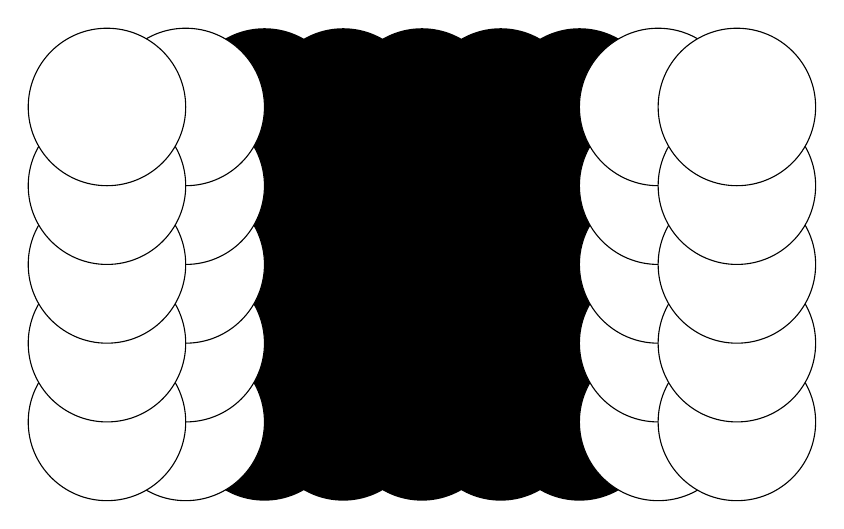
\begin{tikzpicture}
            \draw[very thin, step=1] (0,0) grid(4,4);
            \draw[very thin, dashed,step=1] (-1,0) grid(-2.5,4);
            \draw[very thin, dashed,step=1] (5,0) grid(6.5,4);
            \foreach \x in {0,...,4}{
                \foreach \y in {0,...,4}{
                    \fill (\x,\y) circle(\radius);
                }
            }
            \foreach \x in {-1,-2,5,6}{
                \foreach \y in {0,...,4}{
                    \filldraw[fill=white] (\x,\y) circle(\radius);
                }
            }

        \end{tikzpicture}
        \caption{Normally, one processor only has a local lattice and no data from the neighboring sub-lattices. An empty copy of the sub-lattice is made, to store the shifted lattice.}
    \end{subfigure}
    \begin{subfigure}{\textwidth}
        \centering
        \begin{tikzpicture}
            % Motion
            \draw[very thin, step=1] (0,0) grid(4,4);
            \draw[very thin, dashed,step=1] (-1,0) grid(-2.5,4);
            \draw[very thin, dashed,step=1] (5,0) grid(6.5,4);
            \foreach \x in {0,...,4}{
                \foreach \y in {0,...,4}{
                    \fill (\x,\y) circle(\radius);
                }
            }
            \foreach \x in {-1,-2,5,6}{
                \foreach \y in {0,...,4}{
                    \filldraw[fill=white] (\x,\y) circle(\radius);
                }
            }
            \foreach \x in {0,...,5}{
                \foreach \y in {0,...,4}{
                    \draw (\x,\y) ++(\outbend:\sepradius) coordinate(A);
                    \draw (\x-1,\y) ++(\inbend:\sepradius) coordinate (B);
                    \path[->] (A)  edge[bend right=\inbend] (B);
                }
            }
            \foreach \x in {0,4}{
                \draw (\x-\ovalspacing,-\radius) coordinate (A);
                \draw (A) ++(0,4+2*\radius) coordinate (B);
                \draw (\x+\ovalspacing,-\radius) coordinate (C);
                \draw (C) ++(0,4+2*\radius) coordinate (D);
                \draw[gray] (A) -- (B);
                \draw[gray] (C) -- (D);
                \draw[gray] (A) arc(180:360:\ovalspacing);
                \draw[gray] (D) arc(0:180:\ovalspacing);
            }
        \end{tikzpicture}
        \caption{The shifted lattice is filled with the neighboring links, some of which are received by the ``forward'' neighbor (so some are sent as well to the ``backward'' neighbor)}
        \label{subfig:shift}
    \end{subfigure}
    \begin{subfigure}{\textwidth}
        \centering
        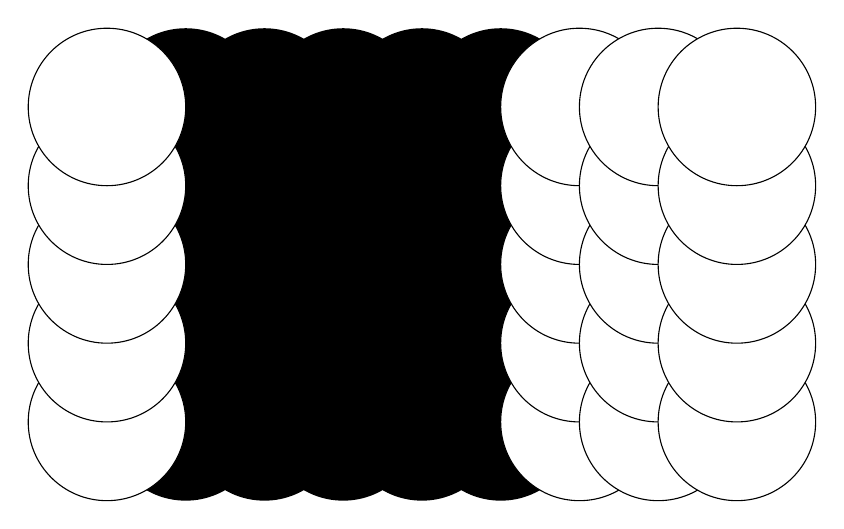
\begin{tikzpicture}
            \draw[very thin, step=1] (0,0) grid(4,4);
            \draw[very thin, dashed,step=1] (-1,0) grid(-2.5,4);
            \draw[very thin, dashed,step=1] (5,0) grid(6.5,4);
            \foreach \x in {-1,...,3}{
                \foreach \y in {0,...,4}{
                    \fill (\x,\y) circle(\radius);
                }
            }
            \foreach \x in {-2,4,5,6}{
                \foreach \y in {0,...,4}{
                    \filldraw[fill=white] (\x,\y) circle(\radius);
                }
            }
        \end{tikzpicture}
        \caption{The shifted lattice is now a local object mapped with the same indices as the original one. A site-by-site multiplication is now possible between the original and the shifted lattices.}
    \end{subfigure}
    \caption{Parallelization scheme based on lattice shifts. When, for example in the staples computation, a link needs to be multiplied by a neighboring one, a new lattice is created. It is filled with the shifted links, which are fetched either from the local sub-lattice if they are the central region, or from the neighbors they are on the edge. This schematic drawing shows how a shift along the ``right'' direction is performed. A new lattice containing the data of the target link is created by filling it with the target links. The circled regions in \cref{subfig:shift}, the edges, are shared using \texttt{MPI} by first creating a ``buffer'' of the shape of the edge (it is a cube in the real simulation) and it is sent in a single message to the neighbor which unpacks it in the right location. The new lattice is then used for arithmetical opertions with the original one on a site by site basis, which now is only a local operation.}
    \label{fig:shift}
\end{figure}

The data to be shifted is on the order of hundreds of kilobytes and sending such an amount of data using \texttt{MPI} is a time consuming operation. A possible optimization that has been implemented is to rewrite the algorithm in order to use non-blocking communications. These allow the program, while the Message Passing Interface is handling the communication, to continue with the execution instead of waiting for the message to be sent. One must however be careful not to use any of the data that is being sent or received before checking that communication has been finished. \\
In the case of lattice shifts the use of non-blocking communications is simple and highly beneficial. 
First let us recall that, because of periodic boundary conditions, sending operations are always paired to a receive one. This means that a processor sends data to its neighbor on one side and receives the corresponding data from the neighbor on the other side along the same direction (this becomes clearer by looking at \cref{fig:shift}). To start a lattice shift one first instantiates a non-blocking send instruction, then shifts the inner points of the sub-lattice (which do not require links from the neighbors) while the message is being sent. To complete the shift operation the last thing to do is to wait for the message from the neighbor from the receiving side to arrive.\\
The great reduction in communication overhead, compared to the single link exchange in \cref{sec:para_gen}, improved the scaling of the algorithm greatly, making this part of the problem much more efficient.

\subsection{Summary of the Parameters for the Gradient Flow}
As it has been done for the gauge field configuration generation algorithm, in \cref{FLOW:params} we report a summary of all free parameters of the program that performs the numerical integration of the gradient flow equation on the lattice.

\begin{table}[!htb]
\begin{center}
    \capt{Parameters for the numerical integration of the gradient flow equations \\on Yang-Mills gauge field configurations.} 
\begin{tabular}{cl}
    Parameter & Description\\\hline
    $\beta$ & Coupling parameter of the Wilson Action, fixed by the input configuration\\
    $\epsilon$ & Runge-Kutta integration step size\\
    $t_f^{MAX}$ & Maximum value of the flow time reached for every configuration. 
\end{tabular}
\label{FLOW:params}
\end{center}
\end{table} 


\section{Structure and Tools}
The programs that have been developed to genereate gauge fields and to apply the gradient flow to them have been written in \texttt{C++}. The full code can be found on the web under the link \url{https://github.com/GioPede}, where source code for both is hosted. The technical documentation is found at \url{https://giopede.github.io/LatticeYangMills/html/index.html}, but it should be noted that this is still in active development, though sufficient for this thesis, so the structure of the source code might vary from what is presented in this section. \\
The choice of programming language was mainly due to it being the most high-performing language with a high enough abstraction level. The high performance of \cpp is given by the tight link that it has to the hardware, allowing precise management of the memory and instructions optimizations. \\
One of the main features that distinguishes \cpp from the \texttt{C} programming language (a valid and equally performing alternative), is that it is an Object-Oriented language. This allows to create abstractions that give an organized structure to the source code, making the developing process easier and the code more readable and intuitive.

\subsection{Object-Oriented Programming}
One of the most successful programming paradigms is Object-Oriented Programming (OOP). An object, or ``class'', in this context is a collection of data, or ``attributes'', and procedures, ``methods'', that act on them. \\
The greatest advantage of using OOP is the introduction of an abstraction level from simple numerical variables, like integers, floating point variables or arrays, to more complex structures. A simple example of this is the class to represent $\mathrm{SU}(3)$ matrices. Instead of dealing every time with the allocation of $18$ variables ($3\times 3$ both for the real and imaginary parts) one can instantiate a variable of type \texttt{SU3}. This example is also useful to introduce the concept of operator overloading, which fundamentally means to implement mathematical operation between classes, so that objects can be used as basic elements of additions, multiplication and so on.\\
Finally, in OOP the concepts of inheritance and polymorphism are very important. The calculation of the observables is a good example for these. An observable, in the program, has a very well defined behavior and structure, for instance it stores its \texttt{value} and has a method \texttt{compute} that can be called to evaluate it given a gauge field lattice as input. However, the operations to be executed in order to compute the value depend on the observable type. An external class that wants to compute multiple observables should be able to call the \texttt{compute} method without knowing the exact type of the observable. The solution is to create an abstract base class, the observable, that only defines \texttt{value} and \texttt{compute}, but gives no specific implementation. Derived types are then created for each different type that ``inherits'' the general behavior from the base class. For an external class, the derived objects can all be used in the same way even if the exact type is unknown. The actual operations that will be performed however will depend on the derived type; this is called polymorphism.\\

\subsection{Source Code Structure}
It is possible to identify a layered structure in the class hierarchy of the program, outlined in \cref{fig:code_structure}. At the time of writing the actual design of the source-code  differs slightly from what is presented here (some classes are merged together, for example the observables), but development is being done to reach this cleaner and fully modular structure.\\

\fig[0.7]{implementation/classes.pdf}{Class structure of the code, showing the approximative hierarchy between the different components.}{fig:code_structure}

There is a set of ``Core Classes'', the second layer in figure, on top of which all the rest is built:
\begin{itemize} 
    \item the $\mathrm{SU}(3)$ matrix implementation, that specifies basic operation for the most fundamental object of Lattice QCD, the link variables. It also includes the algorithm for generating random matrices and the matrix exponential found in \cref{sec:randommatrix,sec:exponential} 
    \item the Lattice class, which specifies operations on four dimensional grids. In particular it handles most of the parallelization tools to allow distributed memory computation, like on computing clusters. The parallelization is introduced by the use of the Message Passing Interface, \texttt{MPI}, to implement for example the lattice shift function, \cref{sec:shift}.
    \item Input/Output tools, to handle input parameter files, gauge configuration parallel reading and writing, observable output files handling and standard command-line output. For the input files the choice has to write a \texttt{json} parsing class, based on the project found at \cite{_nlohmann/json}, to provide an easier user interface via the usage of a  structured input file.
\end{itemize}

With the tools described just above the main classes of the program were written. These ``Lattice Tools'', the third layer in \cref{fig:code_structure}, represent general physical concepts in Lattice QCD. They are:
\begin{itemize}
    \item the Action abstract base class, of which the Wilson Plaquette action derived type has been implemented, is an object that if given a gauge field lattice can compute: the value of the action at every single lattice site; the staples of a link (for the action derivative and the Metropolis-Hastings algorithm); the action difference of a link if provided with a random transformation for it.
    \item the Observable abstract base class. It contains simply the value of the observable and a method to compute it. The derived types that have been implemented are the Plaquette, the Energy Density and the Topological Charge.  
\end{itemize}
For both of these base classes new derived types could be implemented, extending the capabilities and the use cases of the program. \\
Finally the ``Main Applications'' that have been developed are: the Pure Gauge Field Generator, which is an implementation of the Metropolis-Hastings algorithm as presented in this chapter; the Wilson Flow, a program to apply the gradient flow equation to a set of gauge field configuration and compute observables at every flow-time; a Pure Gauge Field Reader, mainly intended for testing, it is a useful application to view the single links of a lattice configuration.